\begin{figure*}[tb]
  \centering
  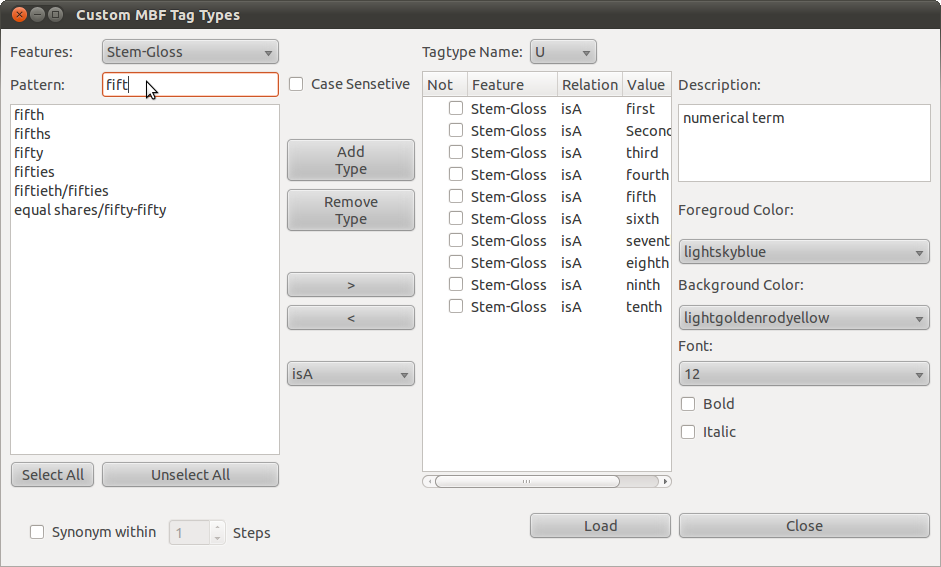
\includegraphics[width=0.9\textwidth]{figures/mbfedit}
  \caption{\framework tag type Boolean formula editor.}
  \label{f:bfe}
\end{figure*}

\framework provides a user friendly interface to specify the 
atomic terms, the \framework Boolean formulae, the \framework regular expressions, 
the tag types, and the legends. 
The \framework GUI also allows the user to modify and correct the 
resulting tag set $R$.
The \framework GUI allows the user also to compute accuracy results 
that compare different tag sets. 
The accuracy results serve well as inter annotation agreement results
when the tag sets come from two human annotators, 
or as evaluation results for learning and information extraction techniques. 

The snapshot in Figure~\ref{f:tagger} shows the \framework GUI with 
the tag type color sensitive view, the tag list view, the tag description view, 
and the match tree. 
In the shown example, the user specified three MBF-based tag types with labels ``HUNDRED'',
``KEY'', and ``DIGITSTENS''. 
The ``HUNDRED'' tag type is based on a simple MBF formula that inspects the gloss tag of 
the stem of the word and checks whether it is {\tt hundred}. 
The ``KEY'' tag type is built on an MBF formula that computes a disjunction 
between the gloss tags of the stems being {\tt thousand/s}, {\tt million/s}, and {\tt billion/s}. 
The ``DIGITSTENS'' tag type is based on a disjunction formula between the gloss tags of the stems 
being {\tt one}, {\tt two},\dots, {\tt ten}, and {\tt twenty}, {\tt thirty},\dots, {\tt ninety}. 
The user also defined an MRE-based tag type with the label ``number''. 
The ``number'' tag type is based on the formula $\left(\textit{HUNDRED}|\textit{KEY}|\textit{DIGITSTENS}\right)+$. 
In words, the formula defines the occurence of one or more consequent tags of the three tags.

The context sensitive menus in Figure~\ref{f:tagger} allow the user to tag 
a selected word or chunk differently or to entirely remove the tag.

The \framework GUI also allows manual tag types that are not based on morphological features.
These tags enable the users to build their own reference corpora without 
help from the morphological analyzer. 

\begin{figure*}[tb]
  \centering
  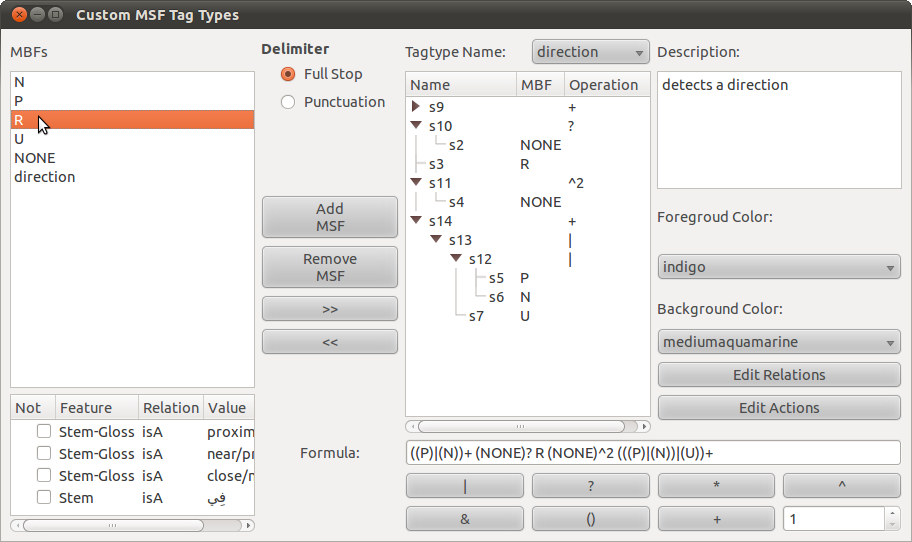
\includegraphics[width=0.9\textwidth]{figures/msfedit}
  \caption{\framework tag type regular expression editor.}
  \label{f:sfe}
\end{figure*}

\subsection{Tag type Boolean formula editor}
The morphology based tag type editor shown in Figure~\ref{f:bfe}
allows the user to write a tag type Boolean formula in a user friendly manner. 
The user first specifies atomic terms by selecting 
a feature from ${\cal F}$. 
The pattern is a regular expression that filters the feature values.
This implicitly helps the user specify 
an {\em exact} versus a {\em partial} match of the  desired 
morphological feature value.

Then the user can add the selected feature values to the atomic terms 
under the tag type name. 
The feature column has a context sensitive menu that allows negating 
the term.
The value column has a context sensitive menu that can switch the 
operation between the values in 
${\cal O} = \{ \mathit{isA}, \mathit{contains}\}$.
The right pane shows a description of the tag type and a set of legend 
descriptors. 

For example, the user can select the feature {\em category} and associate it 
with the value {\em temporal unit}. 
Multiple feature/value pairs can be included in a single tag type 
definition with a disjunction semantics. 

\subsection{Tag type regular expression editor}
The morphology based tag type editor shown in Figure~\ref{f:sfe} allows the 
user to define a tag type regular expression in a user friendly manner. 
The user first adds the required MREs to the formula under the tag type name 
by selecting a label from ${\cal T}$ under MBFs. 
The Boolean formula of a highlighted tag type is shown in the table on the lower left pane. 
Each selected label is associated with an automatic name. 
The regular expression tree features the name, label, and operation for each member MRE.

{\tt NONE} is a special tag type with no Boolean formula. 
It tags all the words that are not tagged with any of the morphology based tag types. 
{\tt NONE} is defined by default and can be used to introduce flexibility and noise tolerance into the formula. 
Moreover, a defined MRE is directly added to the MRE list enabling recursion 
in formula definition. 


Then, the user can construct the formula by applying operations to the selected MREs. 
To do so, the user selects one or two MREs then selects an operation from the ones shown 
in the lower left of the view. 
Without adding operations, the formula is a sequence of the selected MREs. 
The right pane shows a description of the tag type and a set of legend 
descriptors. 

For example, the user can add the {\tt DIGITSTENS}, {\tt KEY}, and {\tt HUNDRED} MREs to the formula. 
Then, he/she selects the {\tt DIGITSTENS} and {\tt KEY} MREs and apply the disjunction ( $|$ ) 
operation to them. 
Similarly, he/she can apply the disjunction operation to the disjunction MRE formed before and {\tt HUNDRED}. 
Last, the user selects the disjunction formula and applies the Kleene star. 
Thus, we get the regular expression shown in Figure~\ref{f:sfe}.

\begin{figure}[h!]
  \centering
  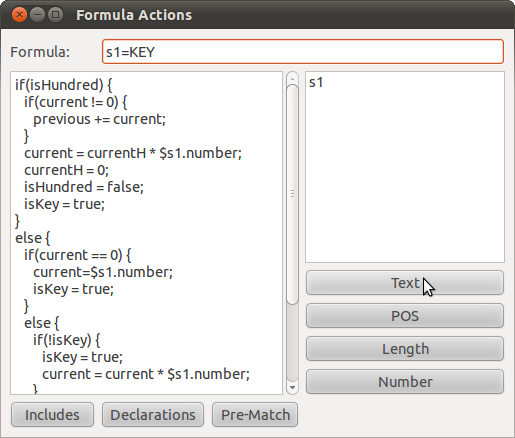
\includegraphics[width=0.45\textwidth]{figures/actions}
  \caption{\framework MRE action sample.}
  \label{f:actions}
\end{figure}

In order to add computational actions to an MRE, 
the user selects to edit the actions in the MRE tag type editor. 
The view shown in Figure~\ref{f:actions} allows the user to specify 
the actions in a user friendly manner. 
\framework enables the user to access the MBF match features easily and define the pre-match actions. 
\framework also enables the user to edit the formula declarations and library includes.

\subsection{Analysis}
In addition to automatic and manual tagging, \framework 
allows comparing tag sets and tag types applied to the
same input text. 
The \framework comparator takes as input two tag sets $R_1$ and $R_2$ and 
two tag type sets ${\cal T}_1$ and ${\cal T}_2$. 
It produces a difference view for the tag types and 
a difference view for the tag sets. 
The tag type difference view shows the common tag types ${\cal T}_1 \cap {\cal T}_2$,
the tag types in ${\cal T}_1$ and not in ${\cal T}_2$, 
and the tag types in ${\cal T}_2$ and not in ${\cal T}_1$.

\begin{figure*}[t]
  \centering
  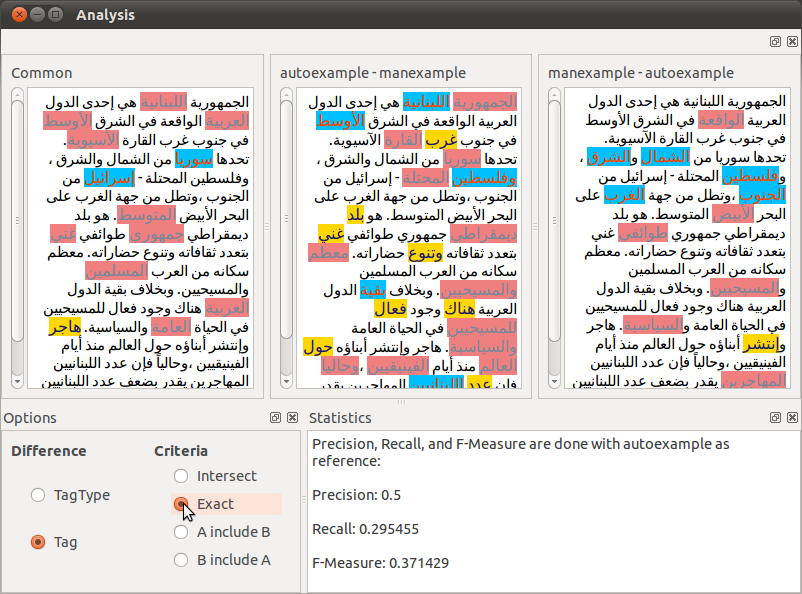
\includegraphics[width=0.9\textwidth]{figures/diff}
  \caption{\framework comparison and accuracy results view.}
  \label{f:diff}
\end{figure*}

Similarly, the tag set difference view shows $R_1\cap R_2$, $R_1/R_2$ and $R_2/R_1$. 
The tag set difference view, as shown in Figure~\ref{f:diff} also shows the precision, 
recall and F-measure between the two sets. 
The metrics can be computed based on several predicates. 
The ``Intersection'' predicate returns true if a tag from $R_1$ intersects in text $T$ 
with a tag in $R_2$. 
The ``Exact'' predicate returns true if a tag from $R_1$ exactly matches a tag
in $R_2$. 
The ``A includes B'' predicate returns true if a tag from $R_1$ contains a tag from $R_2$. 
Finally, the ``B includes A'' predicate returns true if a tag from $R_2$ contains 
a tag from $R_1$. 

In the difference view panes, the user can select a difference tag and accept it, or reject
it to build a corrected corpora. 